% Options for packages loaded elsewhere
\PassOptionsToPackage{unicode}{hyperref}
\PassOptionsToPackage{hyphens}{url}
%
\documentclass[
]{article}
\usepackage{lmodern}
\usepackage{amssymb,amsmath}
\usepackage{ifxetex,ifluatex}
\ifnum 0\ifxetex 1\fi\ifluatex 1\fi=0 % if pdftex
  \usepackage[T1]{fontenc}
  \usepackage[utf8]{inputenc}
  \usepackage{textcomp} % provide euro and other symbols
\else % if luatex or xetex
  \usepackage{unicode-math}
  \defaultfontfeatures{Scale=MatchLowercase}
  \defaultfontfeatures[\rmfamily]{Ligatures=TeX,Scale=1}
\fi
% Use upquote if available, for straight quotes in verbatim environments
\IfFileExists{upquote.sty}{\usepackage{upquote}}{}
\IfFileExists{microtype.sty}{% use microtype if available
  \usepackage[]{microtype}
  \UseMicrotypeSet[protrusion]{basicmath} % disable protrusion for tt fonts
}{}
\makeatletter
\@ifundefined{KOMAClassName}{% if non-KOMA class
  \IfFileExists{parskip.sty}{%
    \usepackage{parskip}
  }{% else
    \setlength{\parindent}{0pt}
    \setlength{\parskip}{6pt plus 2pt minus 1pt}}
}{% if KOMA class
  \KOMAoptions{parskip=half}}
\makeatother
\usepackage{xcolor}
\IfFileExists{xurl.sty}{\usepackage{xurl}}{} % add URL line breaks if available
\IfFileExists{bookmark.sty}{\usepackage{bookmark}}{\usepackage{hyperref}}
\hypersetup{
  pdftitle={Data Visualizations and Analysis},
  pdfauthor={Grayson White},
  hidelinks,
  pdfcreator={LaTeX via pandoc}}
\urlstyle{same} % disable monospaced font for URLs
\usepackage[margin=1in]{geometry}
\usepackage{color}
\usepackage{fancyvrb}
\newcommand{\VerbBar}{|}
\newcommand{\VERB}{\Verb[commandchars=\\\{\}]}
\DefineVerbatimEnvironment{Highlighting}{Verbatim}{commandchars=\\\{\}}
% Add ',fontsize=\small' for more characters per line
\usepackage{framed}
\definecolor{shadecolor}{RGB}{248,248,248}
\newenvironment{Shaded}{\begin{snugshade}}{\end{snugshade}}
\newcommand{\AlertTok}[1]{\textcolor[rgb]{0.94,0.16,0.16}{#1}}
\newcommand{\AnnotationTok}[1]{\textcolor[rgb]{0.56,0.35,0.01}{\textbf{\textit{#1}}}}
\newcommand{\AttributeTok}[1]{\textcolor[rgb]{0.77,0.63,0.00}{#1}}
\newcommand{\BaseNTok}[1]{\textcolor[rgb]{0.00,0.00,0.81}{#1}}
\newcommand{\BuiltInTok}[1]{#1}
\newcommand{\CharTok}[1]{\textcolor[rgb]{0.31,0.60,0.02}{#1}}
\newcommand{\CommentTok}[1]{\textcolor[rgb]{0.56,0.35,0.01}{\textit{#1}}}
\newcommand{\CommentVarTok}[1]{\textcolor[rgb]{0.56,0.35,0.01}{\textbf{\textit{#1}}}}
\newcommand{\ConstantTok}[1]{\textcolor[rgb]{0.00,0.00,0.00}{#1}}
\newcommand{\ControlFlowTok}[1]{\textcolor[rgb]{0.13,0.29,0.53}{\textbf{#1}}}
\newcommand{\DataTypeTok}[1]{\textcolor[rgb]{0.13,0.29,0.53}{#1}}
\newcommand{\DecValTok}[1]{\textcolor[rgb]{0.00,0.00,0.81}{#1}}
\newcommand{\DocumentationTok}[1]{\textcolor[rgb]{0.56,0.35,0.01}{\textbf{\textit{#1}}}}
\newcommand{\ErrorTok}[1]{\textcolor[rgb]{0.64,0.00,0.00}{\textbf{#1}}}
\newcommand{\ExtensionTok}[1]{#1}
\newcommand{\FloatTok}[1]{\textcolor[rgb]{0.00,0.00,0.81}{#1}}
\newcommand{\FunctionTok}[1]{\textcolor[rgb]{0.00,0.00,0.00}{#1}}
\newcommand{\ImportTok}[1]{#1}
\newcommand{\InformationTok}[1]{\textcolor[rgb]{0.56,0.35,0.01}{\textbf{\textit{#1}}}}
\newcommand{\KeywordTok}[1]{\textcolor[rgb]{0.13,0.29,0.53}{\textbf{#1}}}
\newcommand{\NormalTok}[1]{#1}
\newcommand{\OperatorTok}[1]{\textcolor[rgb]{0.81,0.36,0.00}{\textbf{#1}}}
\newcommand{\OtherTok}[1]{\textcolor[rgb]{0.56,0.35,0.01}{#1}}
\newcommand{\PreprocessorTok}[1]{\textcolor[rgb]{0.56,0.35,0.01}{\textit{#1}}}
\newcommand{\RegionMarkerTok}[1]{#1}
\newcommand{\SpecialCharTok}[1]{\textcolor[rgb]{0.00,0.00,0.00}{#1}}
\newcommand{\SpecialStringTok}[1]{\textcolor[rgb]{0.31,0.60,0.02}{#1}}
\newcommand{\StringTok}[1]{\textcolor[rgb]{0.31,0.60,0.02}{#1}}
\newcommand{\VariableTok}[1]{\textcolor[rgb]{0.00,0.00,0.00}{#1}}
\newcommand{\VerbatimStringTok}[1]{\textcolor[rgb]{0.31,0.60,0.02}{#1}}
\newcommand{\WarningTok}[1]{\textcolor[rgb]{0.56,0.35,0.01}{\textbf{\textit{#1}}}}
\usepackage{graphicx,grffile}
\makeatletter
\def\maxwidth{\ifdim\Gin@nat@width>\linewidth\linewidth\else\Gin@nat@width\fi}
\def\maxheight{\ifdim\Gin@nat@height>\textheight\textheight\else\Gin@nat@height\fi}
\makeatother
% Scale images if necessary, so that they will not overflow the page
% margins by default, and it is still possible to overwrite the defaults
% using explicit options in \includegraphics[width, height, ...]{}
\setkeys{Gin}{width=\maxwidth,height=\maxheight,keepaspectratio}
% Set default figure placement to htbp
\makeatletter
\def\fps@figure{htbp}
\makeatother
\setlength{\emergencystretch}{3em} % prevent overfull lines
\providecommand{\tightlist}{%
  \setlength{\itemsep}{0pt}\setlength{\parskip}{0pt}}
\setcounter{secnumdepth}{-\maxdimen} % remove section numbering

\title{Data Visualizations and Analysis}
\author{Grayson White}
\date{7/13/2020}

\begin{document}
\maketitle

\begin{Shaded}
\begin{Highlighting}[]
\KeywordTok{ggplot}\NormalTok{(working_df, }\KeywordTok{aes}\NormalTok{(}\DataTypeTok{x =} \KeywordTok{log}\NormalTok{(pop_}\DecValTok{2018}\NormalTok{), }\DataTypeTok{y =}\NormalTok{ dryDesignFlowMGD)) }\OperatorTok{+}
\StringTok{  }\KeywordTok{geom_point}\NormalTok{() }\OperatorTok{+}
\StringTok{  }\KeywordTok{geom_smooth}\NormalTok{(}\DataTypeTok{method =} \StringTok{"lm"}\NormalTok{, }\DataTypeTok{se =} \OtherTok{FALSE}\NormalTok{) }\OperatorTok{+}
\StringTok{  }\KeywordTok{theme_bw}\NormalTok{() }\OperatorTok{+}
\StringTok{  }\KeywordTok{labs}\NormalTok{(}\DataTypeTok{x =} \StringTok{"Log of Population (2018)"}\NormalTok{)}
\end{Highlighting}
\end{Shaded}

\begin{verbatim}
## `geom_smooth()` using formula 'y ~ x'
\end{verbatim}

\begin{verbatim}
## Warning: Removed 17 rows containing non-finite values (stat_smooth).
\end{verbatim}

\begin{verbatim}
## Warning: Removed 17 rows containing missing values (geom_point).
\end{verbatim}

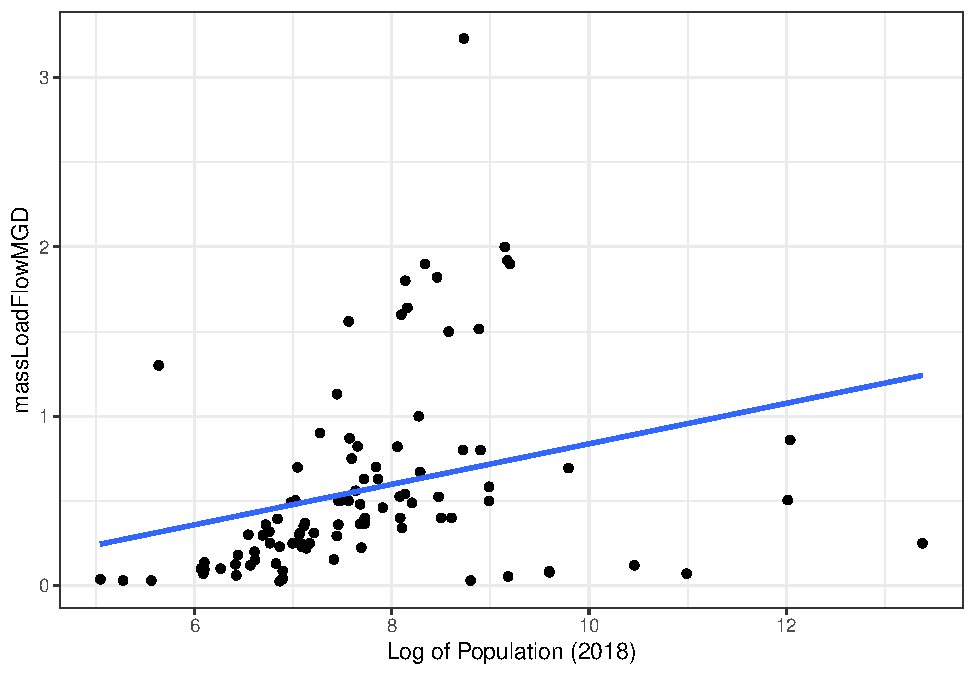
\includegraphics{data-viz_files/figure-latex/unnamed-chunk-2-1.pdf}

\begin{Shaded}
\begin{Highlighting}[]
\KeywordTok{ggplot}\NormalTok{(working_df, }\KeywordTok{aes}\NormalTok{(}\DataTypeTok{x =} \KeywordTok{log}\NormalTok{(pop_}\DecValTok{2018}\NormalTok{),}
                       \DataTypeTok{y =} \KeywordTok{parse_number}\NormalTok{(}\StringTok{`}\DataTypeTok{TSS monthly average lbs/day}\StringTok{`}\NormalTok{))) }\OperatorTok{+}
\StringTok{  }\KeywordTok{geom_point}\NormalTok{() }\OperatorTok{+}
\StringTok{  }\KeywordTok{theme_bw}\NormalTok{()}
\end{Highlighting}
\end{Shaded}

\begin{verbatim}
## Warning: 2 parsing failures.
## row col expected actual
##  13  -- a number     na
##  45  -- a number     na

## Warning: 2 parsing failures.
## row col expected actual
##  13  -- a number     na
##  45  -- a number     na
\end{verbatim}

\begin{verbatim}
## Warning: Removed 19 rows containing missing values (geom_point).
\end{verbatim}

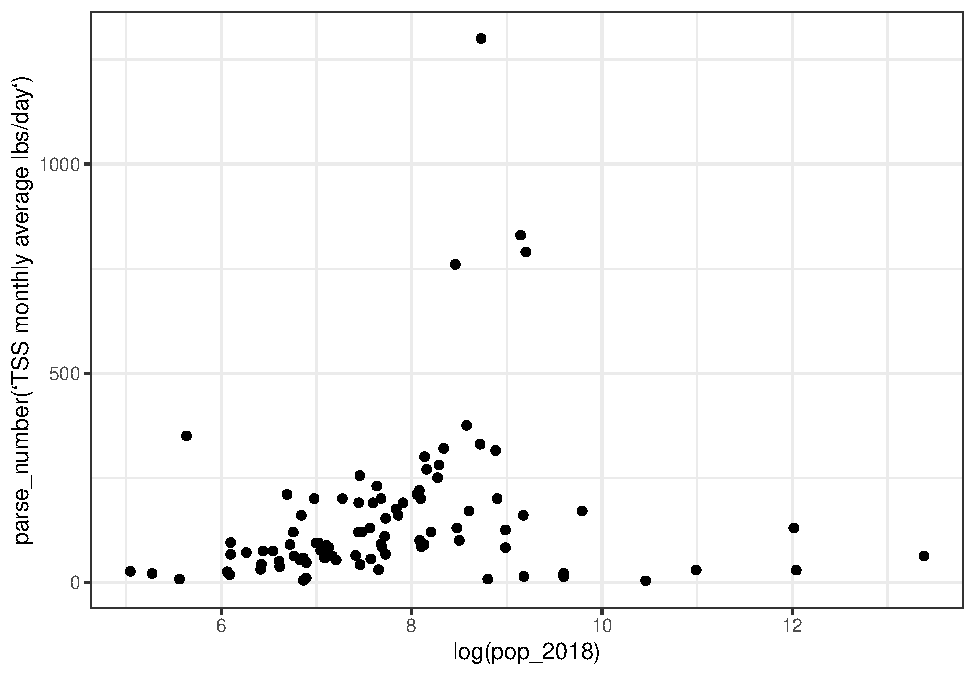
\includegraphics{data-viz_files/figure-latex/unnamed-chunk-3-1.pdf}

\begin{Shaded}
\begin{Highlighting}[]
\NormalTok{working_df }\OperatorTok
\StringTok{  }\KeywordTok{filter}\NormalTok{(type1 }\OperatorTok\StringTok{ }\KeywordTok{c}\NormalTok{(}\StringTok{"lagoons"}\NormalTok{, }\StringTok{"activated sludge"}\NormalTok{)) }\OperatorTok
\StringTok{  }\KeywordTok{group_by}\NormalTok{(type1) }\OperatorTok
\StringTok{  }\KeywordTok{summarize}\NormalTok{(}\DataTypeTok{median =} \KeywordTok{median}\NormalTok{(pop_}\DecValTok{2018}\NormalTok{, }\DataTypeTok{na.rm =} \OtherTok{TRUE}\NormalTok{))}
\end{Highlighting}
\end{Shaded}

\begin{verbatim}
## # A tibble: 2 x 2
##   type1            median
##   <chr>             <dbl>
## 1 activated sludge  1962.
## 2 lagoons           1718.
\end{verbatim}

\begin{Shaded}
\begin{Highlighting}[]
\KeywordTok{library}\NormalTok{(viridis)}
\end{Highlighting}
\end{Shaded}

\begin{verbatim}
## Loading required package: viridisLite
\end{verbatim}

\begin{Shaded}
\begin{Highlighting}[]
\KeywordTok{library}\NormalTok{(plotly)}
\end{Highlighting}
\end{Shaded}

\begin{verbatim}
## 
## Attaching package: 'plotly'
\end{verbatim}

\begin{verbatim}
## The following object is masked from 'package:ggplot2':
## 
##     last_plot
\end{verbatim}

\begin{verbatim}
## The following object is masked from 'package:stats':
## 
##     filter
\end{verbatim}

\begin{verbatim}
## The following object is masked from 'package:graphics':
## 
##     layout
\end{verbatim}

\begin{Shaded}
\begin{Highlighting}[]
\NormalTok{p <-}\StringTok{ }\NormalTok{working_df }\OperatorTok
\StringTok{  }\KeywordTok{ggplot}\NormalTok{(}\KeywordTok{aes}\NormalTok{(}\DataTypeTok{x =}\NormalTok{ Region.x,}
             \DataTypeTok{fill =}\NormalTok{ type1)) }\OperatorTok{+}
\StringTok{  }\KeywordTok{geom_bar}\NormalTok{(}\DataTypeTok{position =} \StringTok{"fill"}\NormalTok{) }\OperatorTok{+}
\StringTok{  }\KeywordTok{scale_fill_viridis_d}\NormalTok{(}\DataTypeTok{option =} \StringTok{"C"}\NormalTok{, }\DataTypeTok{na.value =} \StringTok{"grey50"}\NormalTok{) }\OperatorTok{+}
\StringTok{  }\KeywordTok{scale_x_discrete}\NormalTok{(}\DataTypeTok{labels=}\KeywordTok{c}\NormalTok{(}\StringTok{"Eastern"}\NormalTok{, }\StringTok{"Northwest"}\NormalTok{, }\StringTok{"West"}\NormalTok{)) }\OperatorTok{+}
\StringTok{  }\KeywordTok{theme_bw}\NormalTok{() }\OperatorTok{+}
\StringTok{  }\KeywordTok{labs}\NormalTok{(}\DataTypeTok{x =} \StringTok{"Region"}\NormalTok{,}
       \DataTypeTok{fill =} \StringTok{"Main Type"}\NormalTok{,}
       \DataTypeTok{y =} \StringTok{"Proportion"}\NormalTok{,}
       \DataTypeTok{title =} \StringTok{"Rural WWTPs in Oregon by Type"}\NormalTok{)}
\NormalTok{p}
\end{Highlighting}
\end{Shaded}

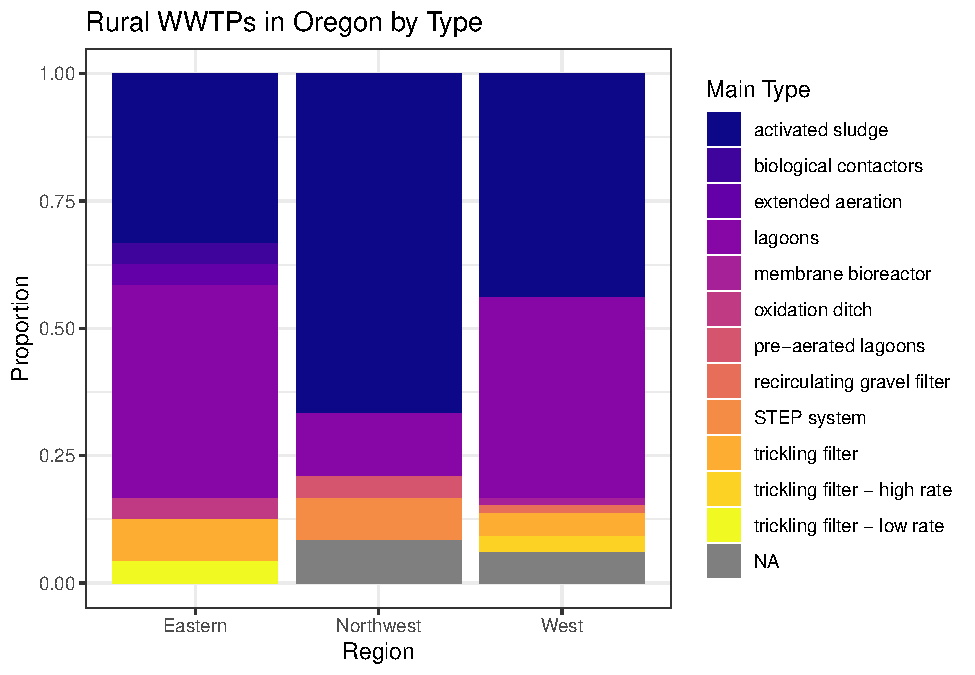
\includegraphics{data-viz_files/figure-latex/unnamed-chunk-5-1.pdf}

\begin{Shaded}
\begin{Highlighting}[]
\CommentTok{# ggplotly(p, tooltip = c("type1", "count"))}

\NormalTok{working_df }\OperatorTok
\StringTok{  }\KeywordTok{filter}\NormalTok{(type2 }\OperatorTok{!=}\StringTok{ }\KeywordTok{c}\NormalTok{(}\StringTok{"na"}\NormalTok{, }\OtherTok{NA}\NormalTok{)) }\OperatorTok
\StringTok{  }\KeywordTok{ggplot}\NormalTok{(}\KeywordTok{aes}\NormalTok{(}\DataTypeTok{x =}\NormalTok{ Region.x,}
             \DataTypeTok{fill =}\NormalTok{ type2)) }\OperatorTok{+}
\StringTok{  }\KeywordTok{geom_bar}\NormalTok{(}\DataTypeTok{position =} \StringTok{"fill"}\NormalTok{) }\OperatorTok{+}
\StringTok{  }\KeywordTok{scale_fill_viridis_d}\NormalTok{(}\DataTypeTok{option =} \StringTok{"C"}\NormalTok{, }\DataTypeTok{na.value =} \StringTok{"grey50"}\NormalTok{) }\OperatorTok{+}
\StringTok{  }\KeywordTok{scale_x_discrete}\NormalTok{(}\DataTypeTok{labels=}\KeywordTok{c}\NormalTok{(}\StringTok{"Eastern"}\NormalTok{, }\StringTok{"Northwest"}\NormalTok{, }\StringTok{"West"}\NormalTok{)) }\OperatorTok{+}
\StringTok{  }\KeywordTok{theme_bw}\NormalTok{() }\OperatorTok{+}
\StringTok{  }\KeywordTok{labs}\NormalTok{(}\DataTypeTok{x =} \StringTok{"Region"}\NormalTok{,}
       \DataTypeTok{fill =} \StringTok{"Secondary Type"}\NormalTok{,}
       \DataTypeTok{y =} \StringTok{"Proportion"}\NormalTok{,}
       \DataTypeTok{title =} \StringTok{"Rural WWTPs in Oregon by Secondary Type"}\NormalTok{)}
\end{Highlighting}
\end{Shaded}

\includegraphics{data-viz_files/figure-latex/unnamed-chunk-5-2.pdf}

\begin{Shaded}
\begin{Highlighting}[]
\KeywordTok{library}\NormalTok{(LaCroixColoR)}

\NormalTok{p4 <-}\StringTok{ }\NormalTok{working_df }\OperatorTok
\StringTok{  }\KeywordTok{mutate}\NormalTok{(}
    \DataTypeTok{type_plot =} \KeywordTok{case_when}\NormalTok{(}
\NormalTok{      type1 }\OperatorTok\StringTok{ }\KeywordTok{c}\NormalTok{(}\StringTok{"lagoons"}\NormalTok{, }\StringTok{"pre-aerated lagoons"}\NormalTok{) }\OperatorTok{~}\StringTok{ "lagoons"}\NormalTok{,}
\NormalTok{      type1 }\OperatorTok\StringTok{ }\KeywordTok{c}\NormalTok{(}\StringTok{"trickling filter"}\NormalTok{, }\StringTok{"trickling filter - high rate"}\NormalTok{,}
                   \StringTok{"trickling filter - low rate"}\NormalTok{) }\OperatorTok{~}\StringTok{ "trickling filter"}\NormalTok{,}
\NormalTok{      type1 }\OperatorTok\StringTok{ }\KeywordTok{c}\NormalTok{(}\StringTok{"activated sludge"}\NormalTok{) }\OperatorTok{~}\StringTok{ "activated sludge"}\NormalTok{,}
\NormalTok{      type1 }\OperatorTok\StringTok{ }\KeywordTok{c}\NormalTok{(}\StringTok{"extended aeration"}\NormalTok{, }\StringTok{"membrane bioreactor"}\NormalTok{, }\StringTok{"recirculating gravel filter"}\NormalTok{, }\OtherTok{NA}\NormalTok{,}
                   \StringTok{"STEP system"}\NormalTok{, }\StringTok{"oxidation ditch"}\NormalTok{, }\StringTok{"biological contactors"}
\NormalTok{    ) }\OperatorTok{~}\StringTok{ "other"}
\NormalTok{  )) }\OperatorTok
\StringTok{  }\KeywordTok{ggplot}\NormalTok{(}\KeywordTok{aes}\NormalTok{(}\DataTypeTok{x =}\NormalTok{ Region.x,}
             \DataTypeTok{fill =} \KeywordTok{factor}\NormalTok{(type_plot, }\DataTypeTok{levels =} \KeywordTok{c}\NormalTok{(}\StringTok{"activated sludge"}\NormalTok{, }\StringTok{"lagoons"}\NormalTok{, }\StringTok{"trickling filter"}\NormalTok{, }\StringTok{"other"}\NormalTok{)))) }\OperatorTok{+}
\StringTok{  }\KeywordTok{geom_bar}\NormalTok{(}\DataTypeTok{position =} \StringTok{"fill"}\NormalTok{) }\OperatorTok{+}
\StringTok{  }\KeywordTok{scale_fill_manual}\NormalTok{(}\DataTypeTok{values =} \KeywordTok{lacroix_palette}\NormalTok{(}\StringTok{"Pamplemousse"}\NormalTok{, }\DataTypeTok{type =} \StringTok{"discrete"}\NormalTok{)) }\OperatorTok{+}
\StringTok{  }\KeywordTok{scale_x_discrete}\NormalTok{(}\DataTypeTok{labels=}\KeywordTok{c}\NormalTok{(}\StringTok{"Eastern"}\NormalTok{, }\StringTok{"Northwest"}\NormalTok{, }\StringTok{"West"}\NormalTok{)) }\OperatorTok{+}
\StringTok{  }\KeywordTok{theme_bw}\NormalTok{() }\OperatorTok{+}
\StringTok{  }\KeywordTok{labs}\NormalTok{(}\DataTypeTok{x =} \StringTok{"Region"}\NormalTok{,}
       \DataTypeTok{fill =} \StringTok{"Type"}\NormalTok{,}
       \DataTypeTok{y =} \StringTok{"Proportion"}\NormalTok{,}
       \DataTypeTok{title =} \StringTok{"Rural WWTPs in Oregon by Type and DEQ Region"}\NormalTok{) }
  \CommentTok{#theme(legend.position = "bottom")}
\NormalTok{p4}
\end{Highlighting}
\end{Shaded}

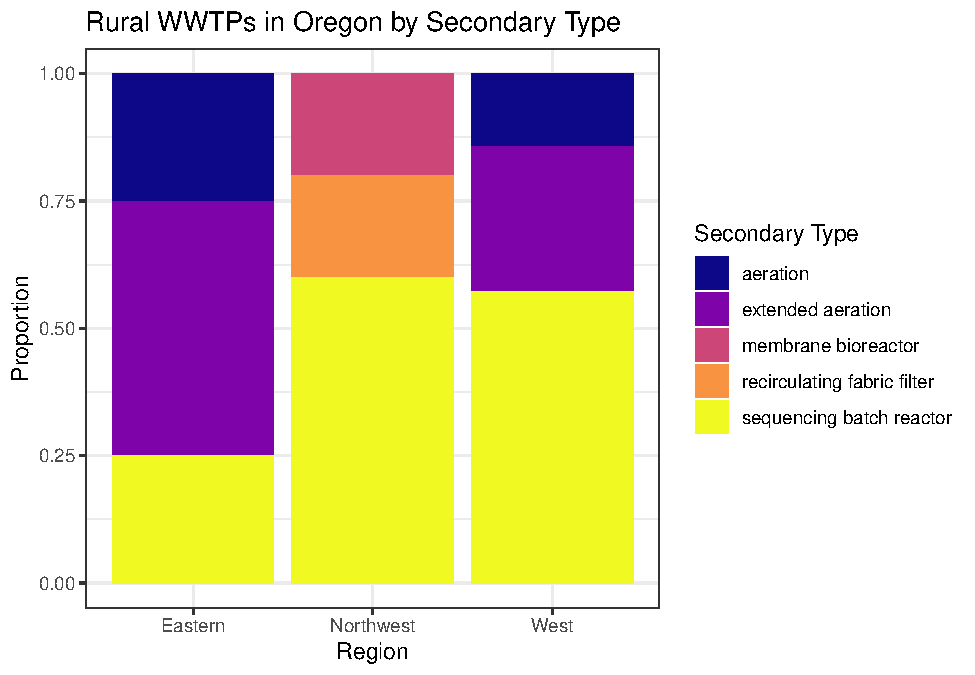
\includegraphics{data-viz_files/figure-latex/unnamed-chunk-5-3.pdf}

\begin{Shaded}
\begin{Highlighting}[]
\KeywordTok{library}\NormalTok{(gtools)}
\NormalTok{working_df}\OperatorTok{$}\NormalTok{quantile_density <-}\StringTok{ }\KeywordTok{quantcut}\NormalTok{(working_df}\OperatorTok{$}\NormalTok{pop_density_}\DecValTok{2018}\NormalTok{, }\DataTypeTok{q =} \DecValTok{4}\NormalTok{)}
\KeywordTok{ggplot}\NormalTok{(working_df[}\OperatorTok{!}\KeywordTok{is.na}\NormalTok{(working_df}\OperatorTok{$}\NormalTok{quantile_density), ], }\KeywordTok{aes}\NormalTok{(}\DataTypeTok{x =}\NormalTok{ quantile_density,}
                       \DataTypeTok{fill =}\NormalTok{ type1)) }\OperatorTok{+}
\StringTok{  }\KeywordTok{geom_bar}\NormalTok{(}\DataTypeTok{position =} \StringTok{"fill"}\NormalTok{) }\OperatorTok{+}
\StringTok{  }\KeywordTok{scale_x_discrete}\NormalTok{(}\DataTypeTok{labels=}\KeywordTok{c}\NormalTok{(}\StringTok{"Up to 1050"}\NormalTok{, }\StringTok{"1050 to 1660"}\NormalTok{, }\StringTok{"1660 to 2350"}\NormalTok{, }\StringTok{"2350 and more"}\NormalTok{)) }\OperatorTok{+}
\StringTok{  }\KeywordTok{scale_fill_viridis_d}\NormalTok{(}\DataTypeTok{option =} \StringTok{"B"}\NormalTok{, }\DataTypeTok{na.value =} \StringTok{"grey50"}\NormalTok{) }\OperatorTok{+}
\StringTok{  }\KeywordTok{theme_bw}\NormalTok{() }\OperatorTok{+}
\StringTok{  }\KeywordTok{theme}\NormalTok{(}\DataTypeTok{axis.text.x =} \KeywordTok{element_text}\NormalTok{(}\DataTypeTok{angle =} \DecValTok{45}\NormalTok{, }\DataTypeTok{vjust =} \DecValTok{1}\NormalTok{, }\DataTypeTok{hjust=}\DecValTok{1}\NormalTok{)) }\OperatorTok{+}
\StringTok{  }\KeywordTok{labs}\NormalTok{(}\DataTypeTok{x =} \StringTok{"Population Density (People / Square Mile)"}\NormalTok{,}
       \DataTypeTok{y =} \StringTok{"Proportion"}\NormalTok{,}
       \DataTypeTok{fill =} \StringTok{"Type"}\NormalTok{,}
       \DataTypeTok{title =} \StringTok{"Types of WWTPs Grouped By Population Density"}\NormalTok{)}
\end{Highlighting}
\end{Shaded}

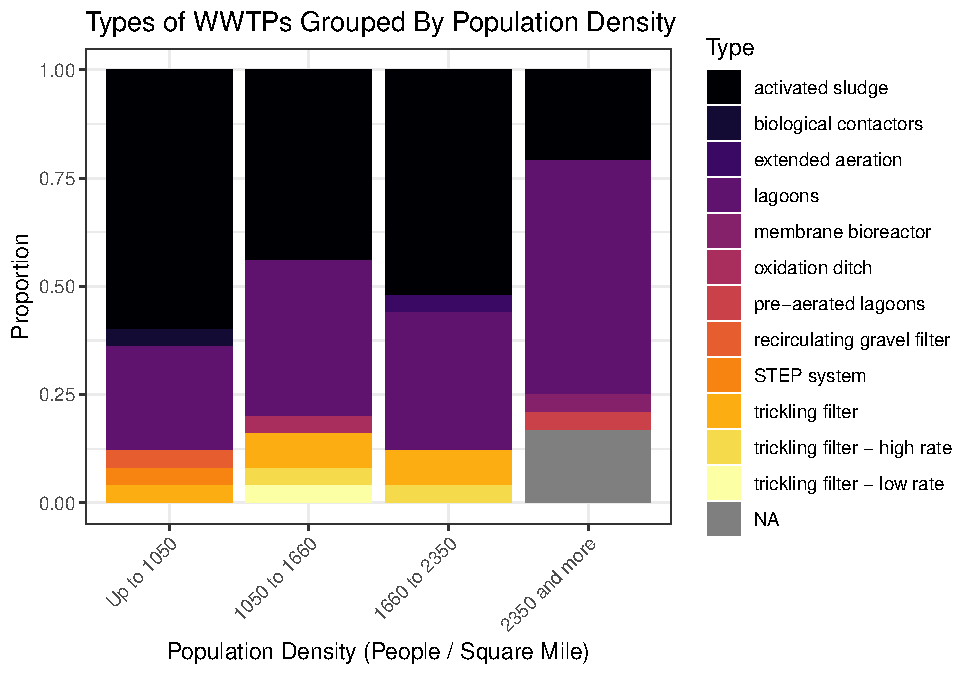
\includegraphics{data-viz_files/figure-latex/unnamed-chunk-6-1.pdf}

\begin{Shaded}
\begin{Highlighting}[]
\NormalTok{working_df}\OperatorTok{$}\NormalTok{quantile_pop_}\DecValTok{2018}\NormalTok{ <-}\StringTok{ }\KeywordTok{quantcut}\NormalTok{(working_df}\OperatorTok{$}\NormalTok{pop_}\DecValTok{2018}\NormalTok{, }\DataTypeTok{q =} \DecValTok{4}\NormalTok{)}
\NormalTok{working_df}\OperatorTok{$}\NormalTok{cut_pop_}\DecValTok{2018}\NormalTok{ <-}\StringTok{ }\KeywordTok{cut}\NormalTok{(working_df}\OperatorTok{$}\NormalTok{pop_}\DecValTok{2018}\NormalTok{, }\DataTypeTok{breaks =} \KeywordTok{c}\NormalTok{(}\DecValTok{0}\NormalTok{, }\DecValTok{2500}\NormalTok{, }\DecValTok{5000}\NormalTok{, }\DecValTok{10000}\NormalTok{, }\FloatTok{1e7}\NormalTok{))}
\NormalTok{p1 <-}\StringTok{ }\KeywordTok{ggplot}\NormalTok{(working_df[}\OperatorTok{!}\KeywordTok{is.na}\NormalTok{(working_df}\OperatorTok{$}\NormalTok{cut_pop_}\DecValTok{2018}\NormalTok{), ], }\KeywordTok{aes}\NormalTok{(}\DataTypeTok{x =}\NormalTok{ cut_pop_}\DecValTok{2018}\NormalTok{,}
                       \DataTypeTok{fill =}\NormalTok{ type1)) }\OperatorTok{+}
\StringTok{  }\KeywordTok{geom_bar}\NormalTok{(}\DataTypeTok{position =} \StringTok{"fill"}\NormalTok{) }\OperatorTok{+}
\StringTok{  }\KeywordTok{scale_x_discrete}\NormalTok{(}\DataTypeTok{labels=}\KeywordTok{c}\NormalTok{(}\StringTok{"Up to 2500"}\NormalTok{, }\StringTok{"2500 to 5000"}\NormalTok{, }\StringTok{"5000 to 10000"}\NormalTok{, }\StringTok{"10000 and more"}\NormalTok{)) }\OperatorTok{+}
\StringTok{  }\KeywordTok{theme_bw}\NormalTok{() }\OperatorTok{+}
\StringTok{  }\KeywordTok{theme}\NormalTok{(}\DataTypeTok{axis.text.x =} \KeywordTok{element_text}\NormalTok{(}\DataTypeTok{angle =} \DecValTok{45}\NormalTok{, }\DataTypeTok{vjust =} \DecValTok{1}\NormalTok{, }\DataTypeTok{hjust=}\DecValTok{1}\NormalTok{)) }\OperatorTok{+}
\StringTok{  }\KeywordTok{labs}\NormalTok{(}\DataTypeTok{x =} \StringTok{"Population (2018)"}\NormalTok{,}
       \DataTypeTok{y =} \StringTok{"Proportion"}\NormalTok{,}
       \DataTypeTok{title =} \StringTok{"Type of WWTP Grouped by Population"}\NormalTok{,}
       \DataTypeTok{fill =} \StringTok{"Type"}\NormalTok{)}

\NormalTok{p1}
\end{Highlighting}
\end{Shaded}

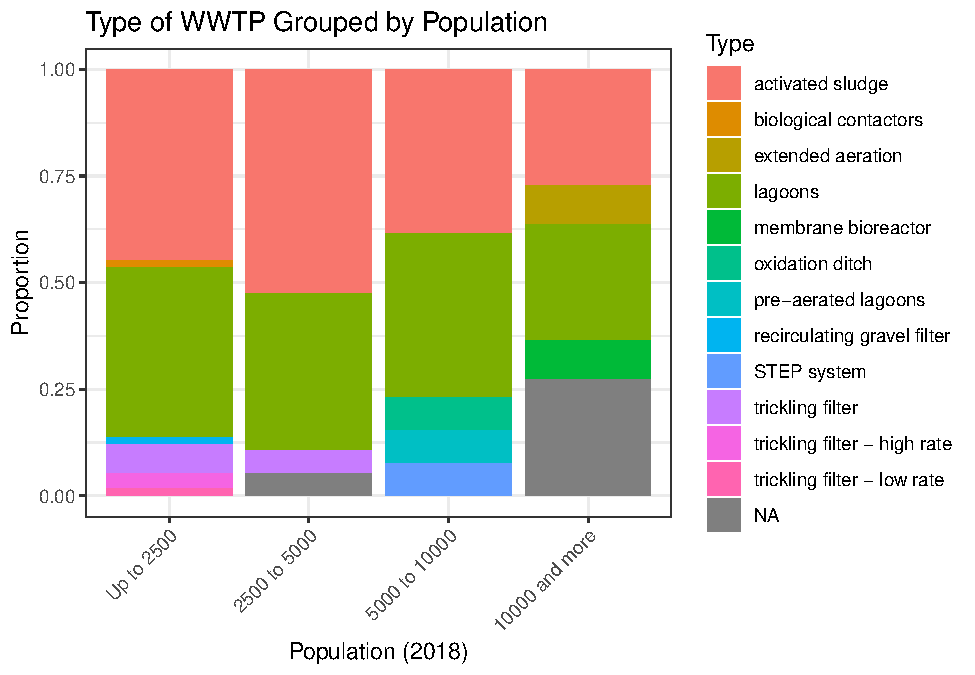
\includegraphics{data-viz_files/figure-latex/unnamed-chunk-6-2.pdf}

\begin{Shaded}
\begin{Highlighting}[]
\CommentTok{# ggplotly(p1)}
\end{Highlighting}
\end{Shaded}

Maps:

\begin{Shaded}
\begin{Highlighting}[]
\KeywordTok{library}\NormalTok{(sf)}
\end{Highlighting}
\end{Shaded}

\begin{verbatim}
## Linking to GEOS 3.6.1, GDAL 2.2.3, PROJ 4.9.3
\end{verbatim}

\begin{Shaded}
\begin{Highlighting}[]
\KeywordTok{library}\NormalTok{(USAboundaries)}
\KeywordTok{library}\NormalTok{(PNWColors)}
\NormalTok{df_sf <-}\StringTok{ }\KeywordTok{st_as_sf}\NormalTok{(working_df, }\DataTypeTok{coords =} \KeywordTok{c}\NormalTok{(}\StringTok{"Longitude"}\NormalTok{, }\StringTok{"Latitude"}\NormalTok{), }\DataTypeTok{crs =} \StringTok{"+proj=longlat +datum=WGS84"}\NormalTok{)}
\NormalTok{OR_sf <-}\StringTok{ }\KeywordTok{us_boundaries}\NormalTok{(}\DataTypeTok{type =} \StringTok{"state"}\NormalTok{, }\DataTypeTok{states =} \StringTok{"OR"}\NormalTok{)}


\NormalTok{working_df_ <-}\StringTok{ }\NormalTok{working_df }\OperatorTok
\StringTok{  }\KeywordTok{filter}\NormalTok{(dryDesignFlowMGD }\OperatorTok{<=}\StringTok{ }\DecValTok{1}\NormalTok{)}
\NormalTok{p2 <-}\StringTok{ }\KeywordTok{ggplot}\NormalTok{() }\OperatorTok{+}
\StringTok{  }\KeywordTok{geom_sf}\NormalTok{(}\DataTypeTok{data =}\NormalTok{ OR_sf, }\DataTypeTok{fill =} \StringTok{"#009474"}\NormalTok{) }\OperatorTok{+}
\StringTok{  }\KeywordTok{geom_point}\NormalTok{(}\DataTypeTok{data =}\NormalTok{ working_df_,}
             \KeywordTok{aes}\NormalTok{(}
                 \DataTypeTok{x =}\NormalTok{ Longitude,}
                 \DataTypeTok{y =}\NormalTok{ Latitude,}
                 \DataTypeTok{size =}\NormalTok{ dryDesignFlowMGD}
\NormalTok{                 ),}
             \DataTypeTok{alpha =} \FloatTok{0.6}\NormalTok{,}
             \DataTypeTok{color =} \StringTok{"#15266B"}\NormalTok{) }\OperatorTok{+}
\StringTok{  }\KeywordTok{coord_sf}\NormalTok{() }\OperatorTok{+}
\StringTok{  }\KeywordTok{theme_void}\NormalTok{() }\OperatorTok{+}
\StringTok{  }\KeywordTok{labs}\NormalTok{(}\DataTypeTok{title =} \StringTok{"Small (<1 MGD) Wastewater Treatment Facilities in Oregon"}\NormalTok{,}
       \DataTypeTok{size =} \StringTok{"Dry Design Flow (MGD)"}\NormalTok{) }\OperatorTok{+}
\StringTok{  }\KeywordTok{theme}\NormalTok{(}\DataTypeTok{plot.title =} \KeywordTok{element_text}\NormalTok{(}\DataTypeTok{hjust =} \FloatTok{0.5}\NormalTok{),}
        \DataTypeTok{plot.title.position =} \StringTok{"plot"}\NormalTok{,}
        \DataTypeTok{legend.position =} \StringTok{"bottom"}\NormalTok{)}

\NormalTok{p2}
\end{Highlighting}
\end{Shaded}

\includegraphics{data-viz_files/figure-latex/unnamed-chunk-7-1.pdf}

\begin{Shaded}
\begin{Highlighting}[]
\CommentTok{# pop la croix}
\NormalTok{working_df <-}\StringTok{ }\NormalTok{working_df }\OperatorTok
\StringTok{  }\KeywordTok{mutate}\NormalTok{(}
    \DataTypeTok{type_plot =} \KeywordTok{case_when}\NormalTok{(}
\NormalTok{      type1 }\OperatorTok\StringTok{ }\KeywordTok{c}\NormalTok{(}\StringTok{"lagoons"}\NormalTok{, }\StringTok{"pre-aerated lagoons"}\NormalTok{) }\OperatorTok{~}\StringTok{ "lagoons"}\NormalTok{,}
\NormalTok{      type1 }\OperatorTok\StringTok{ }\KeywordTok{c}\NormalTok{(}\StringTok{"trickling filter"}\NormalTok{, }\StringTok{"trickling filter - high rate"}\NormalTok{,}
                   \StringTok{"trickling filter - low rate"}\NormalTok{) }\OperatorTok{~}\StringTok{ "trickling filter"}\NormalTok{,}
\NormalTok{      type1 }\OperatorTok\StringTok{ }\KeywordTok{c}\NormalTok{(}\StringTok{"activated sludge"}\NormalTok{) }\OperatorTok{~}\StringTok{ "activated sludge"}\NormalTok{,}
\NormalTok{      type1 }\OperatorTok\StringTok{ }\KeywordTok{c}\NormalTok{(}\StringTok{"extended aeration"}\NormalTok{, }\StringTok{"membrane bioreactor"}\NormalTok{, }\StringTok{"recirculating gravel filter"}\NormalTok{, }\OtherTok{NA}\NormalTok{,}
                   \StringTok{"STEP system"}\NormalTok{, }\StringTok{"oxidation ditch"}\NormalTok{, }\StringTok{"biological contactors"}
\NormalTok{    ) }\OperatorTok{~}\StringTok{ "other/NA"}
\NormalTok{  ))}
\KeywordTok{ggplot}\NormalTok{(working_df[}\OperatorTok{!}\KeywordTok{is.na}\NormalTok{(working_df}\OperatorTok{$}\NormalTok{cut_pop_}\DecValTok{2018}\NormalTok{), ], }\KeywordTok{aes}\NormalTok{(}\DataTypeTok{x =}\NormalTok{ cut_pop_}\DecValTok{2018}\NormalTok{,}
                       \DataTypeTok{fill =} \KeywordTok{factor}\NormalTok{(type_plot, }\DataTypeTok{levels =} \KeywordTok{c}\NormalTok{(}\StringTok{"activated sludge"}\NormalTok{, }\StringTok{"lagoons"}\NormalTok{, }\StringTok{"trickling filter"}\NormalTok{, }\StringTok{"other/NA"}\NormalTok{)))) }\OperatorTok{+}
\StringTok{  }\KeywordTok{geom_bar}\NormalTok{(}\DataTypeTok{position =} \StringTok{"fill"}\NormalTok{) }\OperatorTok{+}
\StringTok{  }\KeywordTok{scale_x_discrete}\NormalTok{(}\DataTypeTok{labels=}\KeywordTok{c}\NormalTok{(}\StringTok{"Up to 2500"}\NormalTok{, }\StringTok{"2500 to 5000"}\NormalTok{, }\StringTok{"5000 to 10000"}\NormalTok{, }\StringTok{"10000 and more"}\NormalTok{)) }\OperatorTok{+}
\StringTok{  }\KeywordTok{scale_fill_viridis_d}\NormalTok{(}\DataTypeTok{option =} \StringTok{"E"}\NormalTok{) }\OperatorTok{+}
\StringTok{  }\KeywordTok{theme_bw}\NormalTok{() }\OperatorTok{+}
\StringTok{  }\KeywordTok{theme}\NormalTok{(}\DataTypeTok{axis.text.x =} \KeywordTok{element_text}\NormalTok{(}\DataTypeTok{angle =} \DecValTok{45}\NormalTok{, }\DataTypeTok{vjust =} \DecValTok{1}\NormalTok{, }\DataTypeTok{hjust=}\DecValTok{1}\NormalTok{),}
        \DataTypeTok{legend.position =} \StringTok{"bottom"}\NormalTok{) }\OperatorTok{+}
\StringTok{  }\KeywordTok{labs}\NormalTok{(}\DataTypeTok{x =} \StringTok{"Population (2018)"}\NormalTok{,}
       \DataTypeTok{y =} \StringTok{"Proportion"}\NormalTok{,}
       \DataTypeTok{title =} \StringTok{"Type of WWTP Grouped by Population"}\NormalTok{,}
       \DataTypeTok{fill =} \StringTok{"Type"}\NormalTok{) }
\end{Highlighting}
\end{Shaded}

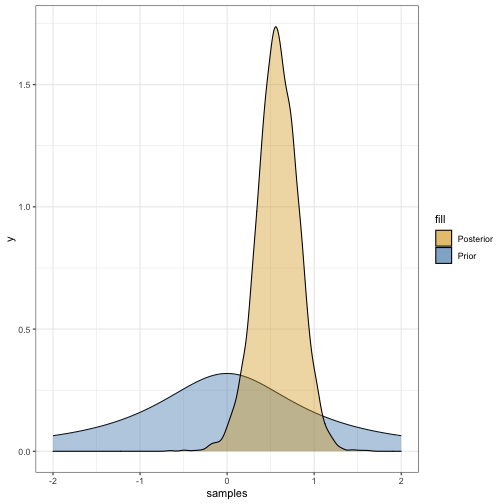
\includegraphics{data-viz_files/figure-latex/unnamed-chunk-8-1.pdf}

\begin{Shaded}
\begin{Highlighting}[]
\CommentTok{# do not run, does not work, crashes R}
\CommentTok{# try pop densities}
\CommentTok{# library(tidycensus)}
\CommentTok{# library(tigris)}
\CommentTok{# }
\CommentTok{# pop_block <- get_acs(}
\CommentTok{#   geography = "block group",}
\CommentTok{#   variables = "B01003_001",}
\CommentTok{#   state = "OR",}
\CommentTok{#   geometry = TRUE,}
\CommentTok{#   key = "abac0e1ca2aa3d3ebb31d6d2fcdbaf52d3e25f7d"}
\CommentTok{# )}
\CommentTok{# }
\CommentTok{# area_2017 <-}
\CommentTok{#   block_groups(year = 2017,}
\CommentTok{#                state = "OR",}
\CommentTok{#                class = "sf")}
\CommentTok{# }
\CommentTok{# area_2017 <- area_2017 %>%}
\CommentTok{#   mutate(area = ALAND / 2589988) %>%}
\CommentTok{#   select(area, geometry, GEOID)}
\CommentTok{# }
\CommentTok{# pop_block <- pop_block %>%}
\CommentTok{#   select(estimate, geometry, GEOID)}
\CommentTok{# }
\CommentTok{# class(pop_block) <- "data.frame"}
\CommentTok{# class(area_2017) <- "data.frame"}
\CommentTok{#     }
\CommentTok{# density <- left_join(pop_block, area_2017, by = c("GEOID" = "GEOID"))}
\CommentTok{# }
\CommentTok{# density <- density %>%}
\CommentTok{#   mutate(pop_density = estimate/area)}
\CommentTok{# }
\CommentTok{# class(density) <- c("sf", "data.frame")}
\end{Highlighting}
\end{Shaded}

\begin{Shaded}
\begin{Highlighting}[]
\NormalTok{working_df }\OperatorTok
\StringTok{  }\KeywordTok{ggplot}\NormalTok{(}\KeywordTok{aes}\NormalTok{(}\DataTypeTok{x =}\NormalTok{ pop_density_}\DecValTok{2018}\NormalTok{)) }\OperatorTok{+}
\StringTok{  }\KeywordTok{geom_density}\NormalTok{(}\DataTypeTok{fill =} \StringTok{"#EBBDCB"}\NormalTok{,}
               \DataTypeTok{alpha =} \FloatTok{0.5}\NormalTok{) }\OperatorTok{+}
\StringTok{  }\KeywordTok{theme_bw}\NormalTok{() }\OperatorTok{+}
\StringTok{  }\KeywordTok{labs}\NormalTok{(}\DataTypeTok{x =} \StringTok{"Population Density (2018)"}\NormalTok{,}
       \DataTypeTok{title =} \StringTok{"Population Density of Towns/Cities in Our Sample"}\NormalTok{)}
\end{Highlighting}
\end{Shaded}

\begin{verbatim}
## Warning: Removed 15 rows containing non-finite values (stat_density).
\end{verbatim}

\includegraphics{data-viz_files/figure-latex/unnamed-chunk-10-1.pdf}

\begin{Shaded}
\begin{Highlighting}[]
\NormalTok{working_df }\OperatorTok
\StringTok{  }\KeywordTok{ggplot}\NormalTok{(}\KeywordTok{aes}\NormalTok{(}\DataTypeTok{x =}\NormalTok{ pop_density_}\DecValTok{2018}\NormalTok{)) }\OperatorTok{+}
\StringTok{  }\KeywordTok{geom_histogram}\NormalTok{(}\DataTypeTok{bins =} \DecValTok{11}\NormalTok{,}
                 \DataTypeTok{fill =} \StringTok{"#EBBDCB"}\NormalTok{,}
                 \DataTypeTok{color =} \StringTok{"grey30"}\NormalTok{) }\OperatorTok{+}
\StringTok{  }\KeywordTok{theme_bw}\NormalTok{() }\OperatorTok{+}
\StringTok{  }\KeywordTok{labs}\NormalTok{(}\DataTypeTok{x =} \StringTok{"Population Density in 2018 (people/square mile)"}\NormalTok{,}
       \DataTypeTok{title =} \StringTok{"Population Density of Towns/Cities in Our Sample"}\NormalTok{)}
\end{Highlighting}
\end{Shaded}

\begin{verbatim}
## Warning: Removed 15 rows containing non-finite values (stat_bin).
\end{verbatim}

\includegraphics{data-viz_files/figure-latex/unnamed-chunk-10-2.pdf}

\begin{Shaded}
\begin{Highlighting}[]
\NormalTok{working_df }\OperatorTok
\StringTok{  }\KeywordTok{filter}\NormalTok{(}\OperatorTok{!}\KeywordTok{is.na}\NormalTok{(basin)) }\OperatorTok
\StringTok{  }\KeywordTok{group_by}\NormalTok{(basin) }\OperatorTok
\StringTok{  }\KeywordTok{summarize}\NormalTok{(}\DataTypeTok{mgd =} \KeywordTok{mean}\NormalTok{(dryDesignFlowMGD, }\DataTypeTok{na.rm =} \OtherTok{TRUE}\NormalTok{)) }\OperatorTok
\StringTok{  }\KeywordTok{ggplot}\NormalTok{(}
    \KeywordTok{aes}\NormalTok{(}\DataTypeTok{x =} \KeywordTok{reorder}\NormalTok{(basin, mgd), }\DataTypeTok{y =}\NormalTok{ mgd)}
\NormalTok{  ) }\OperatorTok{+}
\StringTok{  }\KeywordTok{geom_col}\NormalTok{(}\DataTypeTok{fill =} \StringTok{"maroon"}\NormalTok{) }\OperatorTok{+}
\StringTok{  }\KeywordTok{coord_flip}\NormalTok{() }\OperatorTok{+}
\StringTok{  }\KeywordTok{theme_bw}\NormalTok{() }\OperatorTok{+}
\StringTok{  }\KeywordTok{labs}\NormalTok{(}
    \DataTypeTok{x =} \StringTok{"Average Dry Design Flow (MGD)"}\NormalTok{,}
    \DataTypeTok{y =} \StringTok{"Basin"}\NormalTok{,}
    \DataTypeTok{title =} \StringTok{"Average Dry Design Flow, Grouped By Basin"}
\NormalTok{  )}
\end{Highlighting}
\end{Shaded}

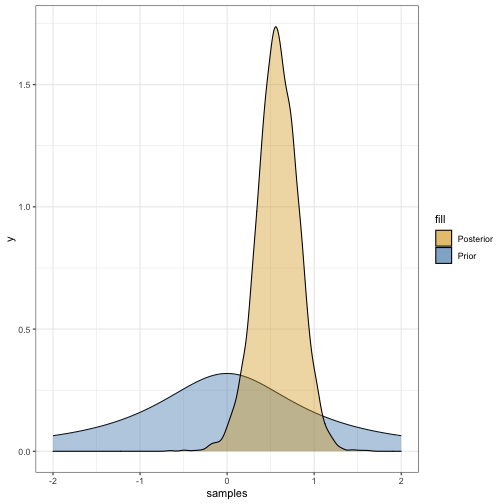
\includegraphics{data-viz_files/figure-latex/unnamed-chunk-11-1.pdf}

\begin{Shaded}
\begin{Highlighting}[]
\CommentTok{# cost}
\NormalTok{cost }\OperatorTok
\StringTok{  }\KeywordTok{ggplot}\NormalTok{(}\KeywordTok{aes}\NormalTok{(}\DataTypeTok{x =} \KeywordTok{log}\NormalTok{(}\StringTok{`}\DataTypeTok{Total Cost}\StringTok{`}\NormalTok{),}
             \DataTypeTok{y =}\NormalTok{ pop_}\DecValTok{2018}\NormalTok{)) }\OperatorTok{+}
\StringTok{  }\KeywordTok{geom_point}\NormalTok{() }\OperatorTok{+}
\StringTok{  }\KeywordTok{theme_bw}\NormalTok{()}
\end{Highlighting}
\end{Shaded}

\begin{verbatim}
## Warning: Removed 2 rows containing missing values (geom_point).
\end{verbatim}

\includegraphics{data-viz_files/figure-latex/unnamed-chunk-12-1.pdf}

\begin{Shaded}
\begin{Highlighting}[]
\NormalTok{cost }\OperatorTok
\StringTok{  }\KeywordTok{ggplot}\NormalTok{(}\KeywordTok{aes}\NormalTok{(}\DataTypeTok{x =} \KeywordTok{log}\NormalTok{(}\StringTok{`}\DataTypeTok{Total Cost}\StringTok{`}\NormalTok{),}
             \DataTypeTok{y =}\NormalTok{ dryDesignFlowMGD)) }\OperatorTok{+}
\StringTok{  }\KeywordTok{geom_point}\NormalTok{() }\OperatorTok{+}
\StringTok{  }\KeywordTok{theme_bw}\NormalTok{()}
\end{Highlighting}
\end{Shaded}

\includegraphics{data-viz_files/figure-latex/unnamed-chunk-12-2.pdf}

\begin{Shaded}
\begin{Highlighting}[]
\NormalTok{cost }\OperatorTok
\StringTok{  }\KeywordTok{ggplot}\NormalTok{(}\KeywordTok{aes}\NormalTok{(}\DataTypeTok{x =} \KeywordTok{log}\NormalTok{(}\StringTok{`}\DataTypeTok{Total Cost}\StringTok{`}\NormalTok{),}
             \DataTypeTok{y =}\NormalTok{ pop_density_}\DecValTok{2018}\NormalTok{)) }\OperatorTok{+}
\StringTok{  }\KeywordTok{geom_point}\NormalTok{() }\OperatorTok{+}
\StringTok{  }\KeywordTok{theme_bw}\NormalTok{()}
\end{Highlighting}
\end{Shaded}

\begin{verbatim}
## Warning: Removed 2 rows containing missing values (geom_point).
\end{verbatim}

\includegraphics{data-viz_files/figure-latex/unnamed-chunk-12-3.pdf}

\begin{Shaded}
\begin{Highlighting}[]
\NormalTok{m1 <-}\StringTok{ }\KeywordTok{lm}\NormalTok{(}\KeywordTok{log}\NormalTok{(}\StringTok{`}\DataTypeTok{Total Cost}\StringTok{`}\NormalTok{) }\OperatorTok{~}\StringTok{ }\NormalTok{dryDesignFlowMGD }\OperatorTok{+}\StringTok{ }\NormalTok{pop_}\DecValTok{2018} \OperatorTok{+}\StringTok{ }\NormalTok{pop_density_}\DecValTok{2018} \OperatorTok{+}\StringTok{ }\NormalTok{Region.x, }\DataTypeTok{data =}\NormalTok{ cost)}
\KeywordTok{summary}\NormalTok{(m1)}
\end{Highlighting}
\end{Shaded}

\begin{verbatim}
## 
## Call:
## lm(formula = log(`Total Cost`) ~ dryDesignFlowMGD + pop_2018 + 
##     pop_density_2018 + Region.x, data = cost)
## 
## Residuals:
##        1        2        3        4        6        7        8       10 
##  0.11565  0.14747 -0.06669  0.04150 -0.04896  0.23982 -0.42879  0.00000 
## 
## Coefficients:
##                    Estimate Std. Error t value Pr(>|t|)   
## (Intercept)      17.1074264  0.6083830  28.119  0.00126 **
## dryDesignFlowMGD -8.5604098  2.3437494  -3.652  0.06746 . 
## pop_2018          0.0008011  0.0001919   4.176  0.05285 . 
## pop_density_2018 -0.0015676  0.0004210  -3.724  0.06515 . 
## Region.xNWR       3.4327461  0.6600789   5.201  0.03504 * 
## Region.xWR        2.7520890  0.7572573   3.634  0.06807 . 
## ---
## Signif. codes:  0 '***' 0.001 '**' 0.01 '*' 0.05 '.' 0.1 ' ' 1
## 
## Residual standard error: 0.3775 on 2 degrees of freedom
##   (2 observations deleted due to missingness)
## Multiple R-squared:  0.9471, Adjusted R-squared:  0.8148 
## F-statistic: 7.158 on 5 and 2 DF,  p-value: 0.1271
\end{verbatim}

\begin{Shaded}
\begin{Highlighting}[]
\KeywordTok{library}\NormalTok{(scales)}
\end{Highlighting}
\end{Shaded}

\begin{verbatim}
## 
## Attaching package: 'scales'
\end{verbatim}

\begin{verbatim}
## The following object is masked from 'package:viridis':
## 
##     viridis_pal
\end{verbatim}

\begin{verbatim}
## The following object is masked from 'package:purrr':
## 
##     discard
\end{verbatim}

\begin{verbatim}
## The following object is masked from 'package:readr':
## 
##     col_factor
\end{verbatim}

\begin{Shaded}
\begin{Highlighting}[]
\NormalTok{point <-}\StringTok{ }\KeywordTok{format_format}\NormalTok{(}\DataTypeTok{big.mark =} \StringTok{","}\NormalTok{, }\DataTypeTok{decimal.mark =} \StringTok{"."}\NormalTok{, }\DataTypeTok{scientific =} \OtherTok{FALSE}\NormalTok{)}
\NormalTok{cost }\OperatorTok
\StringTok{  }\KeywordTok{ggplot}\NormalTok{(}\KeywordTok{aes}\NormalTok{(}\DataTypeTok{x =}\NormalTok{ type1,}
             \DataTypeTok{y =} \KeywordTok{mean}\NormalTok{(}\StringTok{`}\DataTypeTok{Total Cost}\StringTok{`}\NormalTok{))) }\OperatorTok{+}
\StringTok{  }\KeywordTok{geom_col}\NormalTok{(}\DataTypeTok{fill =} \StringTok{"forest green"}\NormalTok{) }\OperatorTok{+}
\StringTok{  }\KeywordTok{labs}\NormalTok{(}\DataTypeTok{x =} \StringTok{"Type of WWTP"}\NormalTok{,}
       \DataTypeTok{y =} \StringTok{"Average Total Cost ($)"}\NormalTok{) }\OperatorTok{+}
\StringTok{  }\KeywordTok{theme_bw}\NormalTok{() }\OperatorTok{+}
\StringTok{  }\KeywordTok{scale_y_continuous}\NormalTok{(}\DataTypeTok{labels =}\NormalTok{ point)}
\end{Highlighting}
\end{Shaded}

\includegraphics{data-viz_files/figure-latex/unnamed-chunk-12-4.pdf}

\begin{Shaded}
\begin{Highlighting}[]
\NormalTok{cost }\OperatorTok
\StringTok{  }\KeywordTok{group_by}\NormalTok{(type1) }\OperatorTok
\StringTok{  }\KeywordTok{summarize}\NormalTok{(}\KeywordTok{n}\NormalTok{())}
\end{Highlighting}
\end{Shaded}

\begin{verbatim}
## # A tibble: 3 x 2
##   type1            `n()`
##   <chr>            <int>
## 1 activated sludge     6
## 2 lagoons              3
## 3 trickling filter     1
\end{verbatim}

\end{document}
